\documentclass[10pt]{beamer}

\usetheme[progressbar=frametitle]{metropolis}
\usepackage{appendixnumberbeamer}
\usepackage[numbers,sort&compress]{natbib}
\bibliographystyle{plainnat}

\usepackage{booktabs}
\usepackage[scale=2]{ccicons}

\usepackage{graphicx}

\usepackage{xspace}
\newcommand{\themename}{\textbf{\textsc{metropolis}}\xspace}

\title{INE5426 AL e AS1}
% \subtitle{Subtítulo}
% \date{\today}
\date{30 de Abril de 2019}
\author{\textbf{João Gabriel Trombeta}  \\
        \textbf{Mathias Olivion Reolon} \\
        \textbf{Otto Menegasso Pires}   \\
        \textbf{Wagner Braga dos Santos}
        }
\institute{Universidade Federal de Santa Catarina - UFSC}
% \titlegraphic{\hfill\includegraphics[height=1.5cm]{logo.pdf}}

\begin{document}

\begin{frame}
    \maketitle
\end{frame}

\begin{frame}{AS1 Questão 1}
    A gramática X++ é recursiva à esquerda?

    \textbf{R:} Não. A definição de uma produção com recursão à esquerda é:
    "expr -> expr + term", e a gramática do X++ não apresenta nenhuma produção
    desse tipo.

   \end{frame}

\begin{frame}{AS1 Questão 1}

    Nota-se de maneira trivial que as produções CLASSDECL, CLASSBODY, VARDECL,
    CONSTRUCTDECL, METHODDECL, METHODBODY, PARAMLIST, PRINTSTAT, READSTAT,
    RETURNSTAT, SUPERSTAT, IFSTAT, FORSTAT, LVALUE, ALOCEXPRESSION, FACTOR não
    são recursivas à esquerda porque em todos os casos a produção mais a
    esquerda é um terminal.

    Para os outros casos é necessário avaliar se não existem recursões indiretas.

\end{frame}

\begin{frame}{AS1 Questão 1}

    PROGRAM não é recursivo pois sua produção leva para CLASSLIST, que leva
    para CLASSDECL, que não é recursiva.

    ATRIBSTAT não é recursivo pois sua produção leva para LVALUE, que não é
    recursiva.

    STATEMENT não é recursivo pois suas produções levam para não-terminais que
    também não possuem recursão.

    STATLIST não é recursivo pois sua produção leva para STATEMENT, que não é
    recursivo.

    EXPRESSION não é recursivo pois sua produção leva para NUMEXPRESSION, que
    leva para TERM, que leva para UNARYEXPR, que leva para FACTOR, que produz
    (EXPRESSION), o que não caracteriza como recursão já que existe o terminal
    ( antes de EXPRESSION.

    ARGLIST não é recursivo pois sua produção leva para EXPRESSION.

\end{frame}

\begin{frame}{AS1 Questão 2}
    A Gramática X++ está fatorada a esquerda? Se não, fatore.

    \textbf{R:} Não, pois existem produções como ALOCEXPRESSION, que ao serem
    expandidas geram coisas como 'new ident ( ARGLIST )' | 'new int ...' | 
    'new string ...' | 'new ident ...'.

    Pode-se perceber que todas as transições a partir de ALOCEXPRESSION se
    iniciam com 'new', sendo que duas delas se iniciam com 'new ident'.
\end{frame}

\begin{frame}{AS1 Questão 2}
    
    Fatoramos ALOCEXPRESSION gerando as seguintes produções:

    ALOCEXPRESSION -> new ALOCEXPRESSION2
    ALOCEXPRESSION2 -> ident ALOCEXPRESSION3 | CTYPE [ EXPRESSION ] ([EXPRESSION])*
    ALOCEXPRESSION3 -> ( ARGLIST ) | [ EXPRESSION ] ([EXPRESSION])*
    CTYPE -> string | int

    Desse modo, para cada produção, não existem duas transições que se iniciam
    com os mesmos terminais ou não terminais.

\end{frame}

\begin{frame}{AS1 Questão 3}
    A gramática X++ é LL(3). Por quê?

    \textbf{R:} Por causa das produções VARDECL e METHODDECL.

\end{frame}

\begin{frame}{AS1 Questão 3}
    VARDECL: Essa produção se inicia com o tipo da variável (int/string/ident).
    Depois tem um identificador que representa o nome da variável e depois
    pode-se ter ou um '[' ou uma ',' ou um ';'. Dependendo do terceiro símbolo
    pode-se ter um ']', completando o '[]', um identificador, declarando uma
    nova variável de mesmo tipo, ou o fim da produção.

    METHODDECL: inicia-se com o tipo do método (int/string/ident), depois pode
    ou não vir uma sequência de '[]' e depois vem o nome do método, em forma de
    ident e finalmente o corpo do método que começa com um '('.

\end{frame}

\begin{frame}{AS1 Questão 3}

    Por causa disso, para se ter certeza que a produção corresponde ou não a um
    VARDECL é preciso olhar 3 símbolos para frente. Por exemplo: Caso os
    primeiros dois símbolos sejam ``int ident'' não é possível saber se é um
    método com o nome ident ou uma variável. Mas ao olhar o terceiro símbolo se
    for ou '[', ou ',', ou ';' então pode-se concluir que se trata de uma
    variável.

\end{frame}

\begin{frame}{AL - AFD}

    A análise é feita utilizando um autômato finito terminístico que reconhece
    os padrões no código. O autômato é descrito em \texttt{automata.txt}, a 
    primeira linha são os estados, a segunda os símbolos, a terceira o estado
    inicial, a quarta o final, e as demais as transições, que devem obedecer o
    padrão \texttt{estado -> destino símbolo}.

    Para facilitar a implementação do lexema pertencente ao token
    \texttt{string\_const}, caso o estado comece com o caracter \texttt{*} o
    autômato irá permanecer no mesmo estado caso ele não possua uma transição
    pelo símbolo lido, ao invés retornar um erro.

\end{frame}

\begin{frame}{AL - Descrição dos estados}

    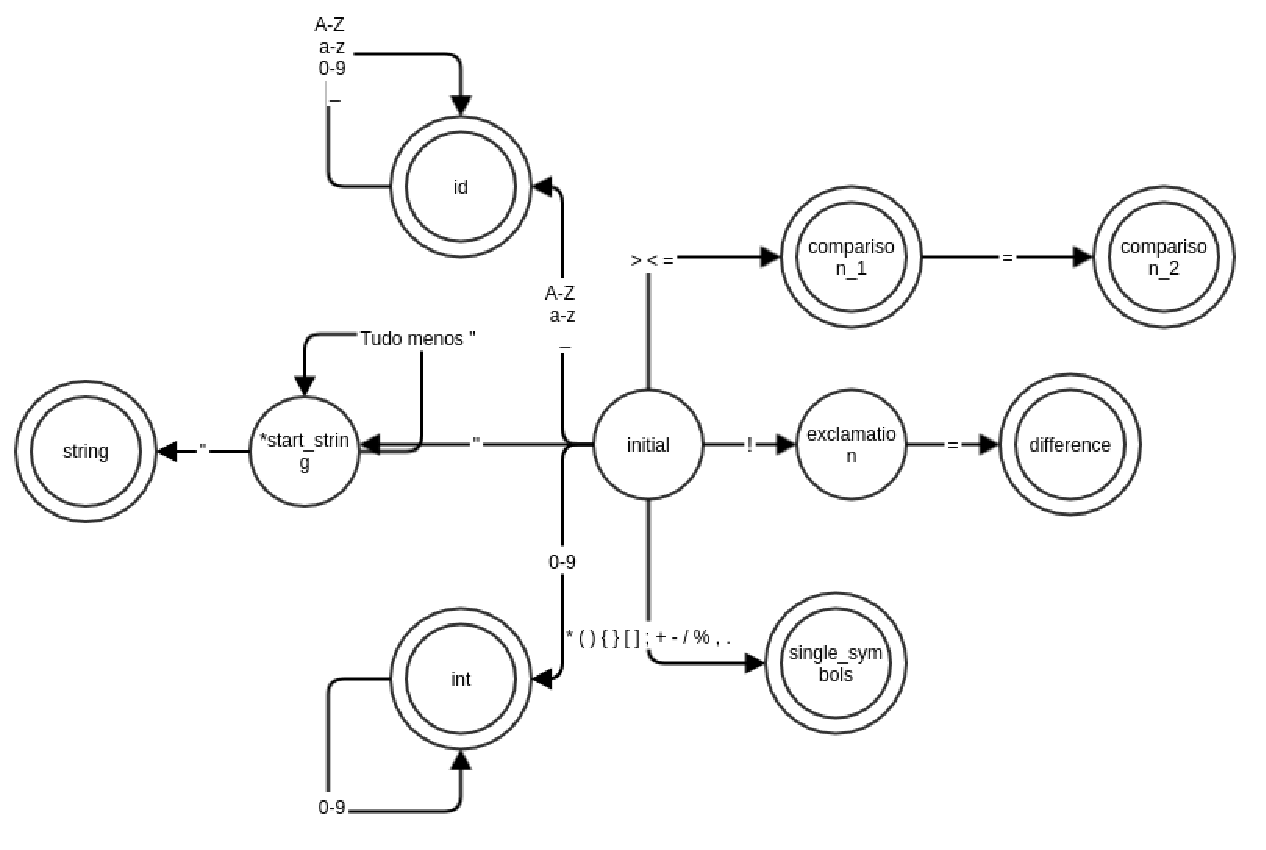
\includegraphics[width=\textwidth,height=\textheight,keepaspectratio]{automata_description.pdf}

\end{frame}

\begin{frame}{AL - \texttt{compiler.py}}

    Instancia o analisador léxico com a descrição do autômato e pede o arquivo
    a ser analisado. O analisador também recebe o conjunto de palavras que são
    palavras reservadas e tipos básicos da linguagem. O analisador então é
    utilizado para gerar todos os tokens.

\end{frame}

\begin{frame}{AL - \texttt{lexical\_analizer.py}}

    O construtor abre o arquivo que descreve o AFD e cria o objeto Automata.
    Ele também abre o código a ser lido e deixa como seu atributo.

    Os tokens são gerados ao chamar \texttt{get\_next\_token}, cada chamada ele
    retorna o próximo token e quando o código acabar ele retorna \texttt{\$}. O
    método ignora brancos e espaçamentos e faz com que o autômato rode sobre o
    arquivo que tem como atributo. Como retorno, a função \texttt{run} do
    autômato informa o estado em que parou, se é de aceitação, e quantos
    símbolosform lidos antes de parar nesse estado. Tendo a informação de
    quantos símbolos foram lidos e o código, o analisador consegue ver o que
    foi lido e cria o token apropriado, colocando-o na tabela de símbolos caso
    necessário. Depois ele atualiza o código de forma a remover o que já foi
    lido e retorna o token.

\end{frame}

\begin{frame}{AL - \texttt{automata.py}}

    Representa o autômato finito. O método \texttt{run} recebe uma string de
    entrada e roda o AFD sobre ela. Caso exista uma transição pelo símbolo lido
    o autômato faz a transição e continua o processo até o momento em lê algo
    inválido. Quando algo inválido é lido o AFD ignora essa leitura e retorna
    o estado atual, se ele é final e quantos símbolos foram lidos. Isso
    acontece porque, por exemplo, tomando a entrada \texttt{" ";}. \texttt{" "}
    é uma entrada válida que leva o autômato pro estado de aceitação
    \texttt{string}, mas quando o símbolo \texttt{;} for lido isso resultaria
    em um erro, uma vez que do estado \texttt{string} não existe mais
    transições. Então \texttt{;} é ignorado e o autômato retorna que leu uma
    string. Quando o método for chamado novamente o AFD estará no estado
    inicial e conseguirá reconhecer \texttt{;} como um padrão válido.

\end{frame}

\end{document}
